\section{Ackerman steering drive}

The most common form of kinematics worldwide involves vehicles equipped with four wheels in motion. 
These wheels are capable of turning but within certain limitations in their angles of rotation. 
Notably, this kinematic system does not incorporate in-place rotation.
\begin{figure}[H]
    \centering
    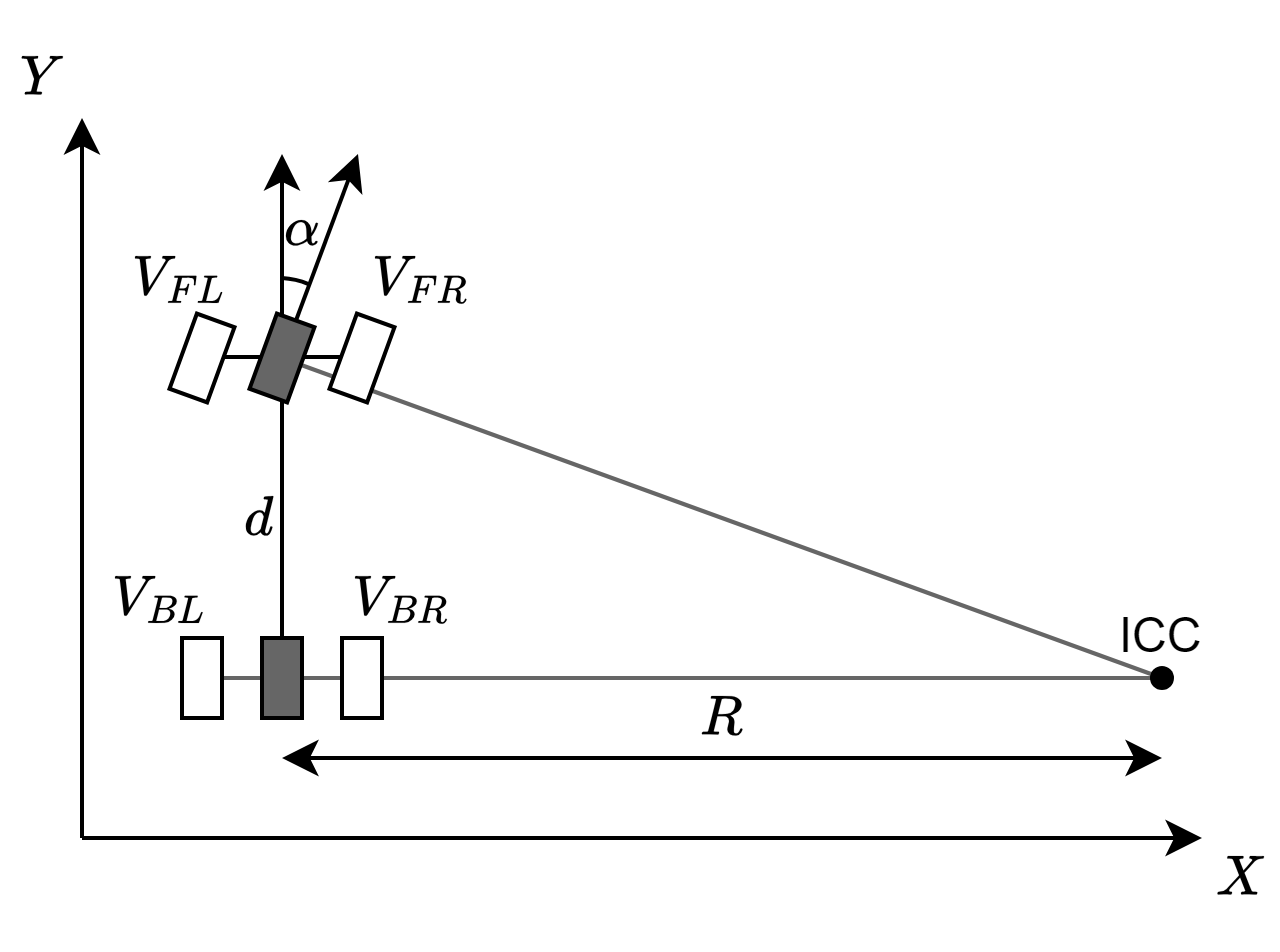
\includegraphics[width=0.5\linewidth]{images/ack.png} 
    \caption{Ackerman steering drive robot}
\end{figure}
We simplify the model to resemble a bicycle:
\[\begin{cases}
    R=\dfrac{d}{\tan\alpha} \\
    \dfrac{\omega d}{\sin\alpha}
\end{cases}\]
This is with reference to the center of actual wheels:
\[\omega R = V \rightarrow \omega=V\dfrac{\tan\alpha}{d}\]